% Chương 1

\chapter{TỔNG QUAN ĐỀ TÀI} % Tên của chương

\label{Chapter1} % Để trích dẫn chương này ở chỗ nào đó trong bài, hãy sử dụng lệnh \ref{Chapter1} 

%----------------------------------------------------------------------------------------

% Định nghĩa một số lệnh cần thiết để điều chỉnh định dạng cho một số nội dung nhất định trong bài
\newcommand{\keyword}[1]{\textbf{#1}}
\newcommand{\tabhead}[1]{\textbf{#1}}
\newcommand{\code}[1]{\texttt{#1}}
\newcommand{\file}[1]{\texttt{\bfseries#1}}
\newcommand{\option}[1]{\texttt{\itshape#1}}

%----------------------------------------------------------------------------------------

\section{Giới thiệu bài toán}

Trong kỷ nguyên của trí tuệ nhân tạo và các hệ thống tự hành, bài toán nhận diện vật cản và ước lượng khoảng cách đã trở thành một trong những hướng nghiên cứu trọng tâm và tiên phong của lĩnh vực Thị giác máy tính (Computer Vision). Ý nghĩa của bài toán này không chỉ dừng lại ở việc tối ưu hóa công nghệ, mà còn mang giá trị nhân văn sâu sắc khi được ứng dụng để xây dựng các hệ thống điều hướng thông minh, hỗ trợ người khiếm thị tái hòa nhập cộng đồng. Đối với người khiếm thị, việc di chuyển trong môi trường thực tế là một thách thức lớn khi xung quanh luôn tồn tại các mối nguy cơ chuyển động liên tục và bất ngờ như người đi bộ, xe máy, ô tô, hoặc các chướng ngại vật tĩnh như cột điện, biển báo, bàn ghế. Một hệ thống trợ thính hoặc trợ thị thông minh không chỉ cần đóng vai trò như một đôi mắt thứ hai để nhận biết môi trường, mà còn phải là một bộ não có khả năng phân tích không gian trong thời gian thực, từ đó đưa ra những chỉ dẫn an toàn và kịp thời cho người dùng.

Để giải quyết trọn vẹn bài toán hỗ trợ điều hướng, hệ thống không thể dựa vào một kỹ thuật đơn lẻ mà phải phối hợp nhịp nhàng một chuỗi các tác vụ phức tạp theo trình tự tuyến tính. Đầu tiên là tác vụ nhận diện đối tượng (Object Detection) nhằm phân tích các khung hình thu nhận từ camera để xác định chính xác danh tính và vị trí của các vật cản xuất hiện trong tầm nhìn. Tiếp theo, tác vụ theo dõi đối tượng (Object Tracking) được thực hiện để duy trì thông tin định danh của từng vật thể xuyên suốt các khung hình liên tiếp, giúp hệ thống hiểu được quỹ đạo và hướng di chuyển của vật cản, đồng thời phân biệt giữa chướng ngại vật tĩnh và động. Cuối cùng, tác vụ ước lượng độ sâu (Depth Estimation) tiến hành đo lường khoảng cách tương đối từ camera đến vật cản, cung cấp dữ liệu số học nền tảng để đánh giá mức độ rủi ro va chạm.

Mặc dù lý thuyết về các mô hình độc lập đã đạt được nhiều bước tiến, việc tích hợp chúng vào một hệ thống hỗ trợ người khiếm thị trong môi trường thực tế vẫn đối mặt với những rào cản kỹ thuật lớn. Sự biến động của môi trường như điều kiện ánh sáng thay đổi thất thường, mật độ giao thông đông đúc, và hiện tượng các vật cản che khuất lẫn nhau dễ làm giảm độ chính xác của mô hình nhận diện. Bên cạnh đó, hệ thống phục vụ người đi lại luôn yêu cầu tốc độ phản hồi cực cao dưới áp lực xử lý thời gian thực, bởi bất kỳ sự trễ nào trong quá trình tính toán đều có thể dẫn đến nguy cơ va chạm thực tế. Ngoài ra, việc lồng ghép nhiều mô hình học sâu (Deep Learning) vào cùng một hệ thống sẽ gây áp lực lớn lên tài nguyên phần cứng, đòi hỏi phải giải quyết triệt để bài toán tối ưu hóa tốc độ xử lý và đồng bộ hóa dữ liệu giữa các luồng thuật toán.

Để vượt qua các thách thức trên, đề tài này đề xuất một giải pháp toàn diện mang tính đột phá dựa trên việc kết hợp các công nghệ tiên tiến nhất hiện nay. Hệ thống sử dụng mô hình YOLO26 làm kiến trúc cốt lõi cho tác vụ nhận diện vật cản nhờ tốc độ xử lý vượt trội và khả năng nhận diện đa lớp vật thể chính xác. Song song với đó, thuật toán ByteTrack được tích hợp để theo dõi đối tượng xuyên khung hình, duy trì quỹ đạo chuyển động ổn định ngay cả khi vật cản bị che khuất tạm thời. Đối với việc tính toán khoảng cách, mô hình MiDaS được ứng dụng để ước lượng độ sâu từ ảnh đơn, cho phép tối ưu chi phí phần cứng mà không cần đến các hệ thống camera kép hay cảm biến đắt đỏ. Cuối cùng, các luồng dữ liệu này được tổng hợp thông qua một thuật toán phân tích mức độ nguy hiểm để phát ra cảnh báo bằng giọng nói tiếng Việt trực quan, hướng tới một giải pháp công nghệ có độ chính xác cao và hoạt động mượt mà trong thời gian thực.

%----------------------------------------------------------------------------------------
\section{Các phương pháp nghiên cứu trước đây}

Trong lĩnh vực nhận diện vật cản và hỗ trợ điều hướng thông minh, việc áp dụng trí tuệ nhân tạo, đặc biệt là các mô hình học sâu (Deep Learning), đã tạo nên những bước đột phá mạnh mẽ. Các nghiên cứu trước đây chủ yếu tập trung vào bài toán phát hiện đối tượng (Object Detection) nhằm xác định đồng thời vị trí và nhãn phân loại của các vật thể trong môi trường. Dựa trên cấu trúc kiến trúc mạng, các phương pháp này được chia thành hai nhóm tiếp cận chính bao gồm bộ dò hai giai đoạn (Two-stage detector) và bộ dò một giai đoạn (One-stage detector). Việc phân tích và đánh giá chi tiết các phương pháp điển hình này là cơ sở lý thuyết quan trọng để định hình giải pháp tối ưu cho hệ thống hỗ trợ người khiếm thị.

\subsection{Phương pháp Faster R-CNN}

Faster R-CNN là mô hình đại diện tiêu biểu và thành công nhất trong nhóm kiến trúc bộ dò hai giai đoạn. Mô hình này ra đời nhằm khắc phục nhược điểm về tốc độ của các phiên bản tiền nhiệm bằng cách loại bỏ thuật toán trích xuất vùng đề xuất truyền thống mang tính thủ công và thay thế bằng một mạng thần kinh tích chập đồng bộ. Quy trình hoạt động của Faster R-CNN được chia làm hai giai đoạn rõ rệt. Trong giai đoạn đầu tiên, hình ảnh đầu vào được xử lý qua một mạng nền tảng để trích xuất ra các bản đồ đặc trưng, sau đó một mạng đề xuất vùng chuyên biệt có tên gọi là Region Proposal Network sẽ tiến hành quét qua bản đồ này để dự đoán xác suất chứa đối tượng và đưa ra các khung hình ứng viên sơ bộ. Sang giai đoạn thứ hai, các vùng đề xuất được chuẩn hóa về một kích thước cố định thông qua lớp RoI Pooling rồi chuyển đến các lớp kết nối đầy đủ để thực hiện song song hai nhiệm vụ là phân loại chính xác nhãn của đối tượng và tinh chỉnh tối ưu tọa độ khung bao cuối cùng.

Nhờ cơ chế tách biệt hai giai đoạn mang tính tuần tự này, Faster R-CNN sở hữu ưu điểm vượt trội về độ chính xác khi nhận diện. Mô hình đặc biệt xuất sắc trong việc phát hiện các vật thể có kích thước nhỏ, cấu trúc phức tạp hoặc các đối tượng bị che khuất một phần trong không gian. Tuy nhiên, nhược điểm lớn nhất của Faster R-CNN lại nằm ở tốc độ suy luận do việc phải xử lý hàng ngàn vùng đề xuất tiêu tốn lượng tài nguyên tính toán cực kỳ lớn. Chính sự hạn chế về mặt tốc độ này khiến mô hình không đạt được tính khả thi khi triển khai trên các thiết bị nhúng cầm tay hoặc các hệ thống yêu cầu phản hồi thời gian thực tức thời như thiết bị hỗ trợ người khiếm thị di chuyển.

\subsection{Phương pháp SSD}

Mô hình SSD (Single Shot MultiBox Detector) được giới thiệu nhằm mục tiêu tối ưu hóa tốc độ xử lý của kiến trúc một giai đoạn nhưng vẫn cố gắng duy trì độ chính xác tiệm cận với các bộ dò hai giai đoạn phức tạp. Cấu trúc và cơ chế hoạt động cốt lõi của SSD được xây dựng dựa trên sự kết hợp của ba thành phần kỹ thuật nền tảng bao gồm mạng nền tảng cơ sở, hệ thống bản đồ đặc trưng đa tỷ lệ và cơ chế khung neo mặc định. 

\begin{figure}[H]
    \centering
    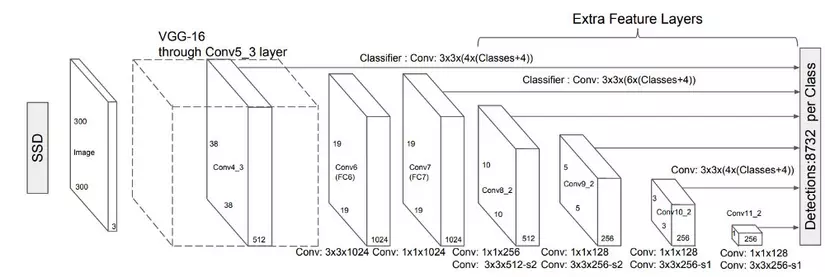
\includegraphics[width=1.0\linewidth]{Figures/Chapter 1/Chapter_2.png}
    \caption{Kiến trúc của phương pháp SSD.}
    \label{fig:ssd_architecture}
\end{figure}

Mạng cơ sở của SSD thường sử dụng kiến trúc VGG-16 hoặc MobileNet đã được loại bỏ các tầng kết nối đầy đủ (Fully Connected Layers) nhằm trích xuất các đặc trưng thô từ hình ảnh đầu vào với chi phí tính toán thấp. Điểm cải tiến lớn nhất của SSD so với các mô hình cùng thời kỳ nằm ở việc bổ sung một chuỗi các tầng tích chập phụ với kích thước giảm dần một cách lũy tiến ngay sau mạng nền tảng, tạo ra một hệ thống các bản đồ đặc trưng đa tỷ lệ (Multi-scale Feature Maps). Quy trình này cho phép mô hình thực hiện dự đoán độc lập trên nhiều tầng mạng khác nhau. Cụ thể, các tầng bản đồ kích thước lớn ở phía nông có độ phân giải không gian cao sẽ chịu trách nhiệm phát hiện các vật thể kích thước nhỏ, trong khi các tầng bản đồ kích thước nhỏ ở phía sâu chứa nhiều hàm lượng thông tin ngữ nghĩa cao cấp sẽ chịu trách nhiệm cấu trúc và phát hiện các vật thể có kích thước lớn hơn. 

\begin{figure}[H]
    \centering
    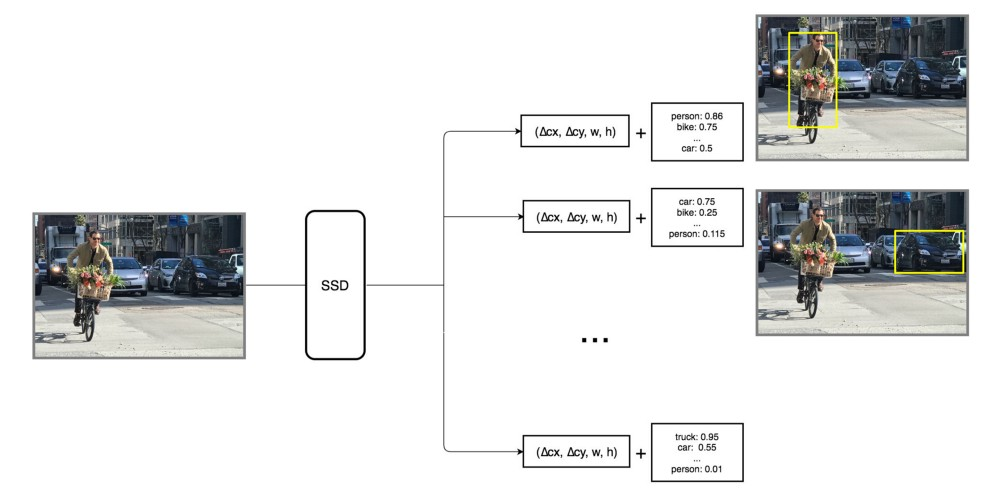
\includegraphics[width=0.9\linewidth]{Figures/Chapter 1/Chapter_1.jpeg}
    \caption{Sơ đồ kiến trúc và cơ chế hoạt động của phương pháp SSD.}
    \label{fig:ssd_architecture}
\end{figure}

Tại mỗi ô lưới trên từng bản đồ đặc trưng đa tỷ lệ này, SSD phân bố một tập hợp các khung neo mặc định (Default Boxes) với nhiều tỷ lệ khía cạnh và kích thước hình học khác nhau. Trong quá trình suy luận, mô hình sẽ tính toán trực tiếp độ lệch tọa độ của khung bao thực tế so với các khung neo mặc định này, đồng thời dự đoán điểm số tin cậy cho từng lớp đối tượng cụ thể. Cuối cùng, hệ thống áp dụng thuật toán triệt tiêu cực đại không giao nhau (Non-Maximum Suppression) để lọc sạch các khung bao chồng chéo và giữ lại kết quả tối ưu nhất.

\subsection*{1. Vấn đề của phương pháp SSD}

Mặc dù SSD (Single Shot MultiBox Detector) là một cột mốc công nghệ quan trọng trong sự phát triển của lĩnh vực thị giác máy tính, việc không lựa chọn mô hình này làm kiến trúc nhận diện cho hệ thống hỗ trợ người khiếm thị xuất phát từ hai nguyên nhân kỹ thuật cốt lõi sau đây.

Nguyên nhân đầu tiên nằm ở sự hạn chế cố hữu về mặt kiến trúc, dẫn đến hiệu năng nhận diện kém đối với các chướng ngại vật nhỏ hoặc nằm ở khoảng cách xa. Đối với người khiếm thị, việc phát hiện sớm các nguy cơ từ xa như cột điện, biển báo, hoặc các vật thể nhỏ dưới lòng đường như viên gạch, hố sụt là yếu tố quyết định đến sự an toàn vật lý trong quá trình di chuyển. Tuy nhiên, cấu trúc của SSD lại thực hiện việc trích xuất đặc trưng và dự đoán theo một chiều thẳng đứng từ nông đến sâu, hoàn toàn thiếu vắng các cơ chế hợp nhất đặc trưng hiện đại như mạng kim tự tháp đặc trưng (Feature Pyramid Network) hay mạng tổng hợp đường dẫn (Path Aggregation Network). Do SSD tiến hành dự đoán các vật thể nhỏ hoàn toàn độc lập dựa trên các tầng mạng nông ban đầu, nơi hàm lượng thông tin ngữ nghĩa còn rất nghèo nàn và mạng chưa hiểu rõ cấu trúc vật thể nên bài toán rất dễ bỏ sót mục tiêu hoặc đưa ra các cảnh báo sai lệch. Ngược lại, các dòng mạng thế hệ mới hiện nay sử dụng cơ chế kết nối ngược linh hoạt, cho phép thông tin ngữ nghĩa cấp cao bổ sung liên tục cho thông tin không gian ở tầng thấp, giải quyết triệt để bài toán nhận diện vật thể đa quy mô mà SSD gặp phải.

Nguyên nhân thứ hai xuất phát từ áp lực tối ưu hóa hiệu năng và tính bất tương thích của SSD khi đặt trong một hệ sinh thái đa tác vụ thời gian thực. Hệ thống đề xuất của đề tài không thuần túy là một bộ dò ảnh đơn lẻ, mà là một phức hợp công nghệ hoạt động đồng thời bao gồm nhận diện vật cản, theo dõi quỹ đạo bằng ByteTrack và ước lượng độ sâu bằng mô hình MiDaS. Bản thân MiDaS là một cấu trúc học sâu từ ảnh đơn tương đối nặng và chiếm dụng nhiều tài nguyên đồ họa; do đó, nếu lựa chọn SSD, hệ thống sẽ buộc phải nâng cấp mạng nền tảng lên cấu hình rất lớn để bù đắp lỗ hổng về độ chính xác, vô tình tạo ra hiện tượng thắt nút cổ chai về mặt hiệu năng và làm sụt giảm nghiêm trọng tốc độ khung hình (FPS) trên các thiết bị nhúng. Bên cạnh đó, SSD thường xuyên gặp hiện tượng rung lắc khung bao (bounding box jittering) khi đối tượng chuyển động nhanh. Nhược điểm này trực tiếp phá vỡ tính ổn định của thuật toán ByteTrack — vốn là liên kết phụ thuộc chặt chẽ vào độ tin cậy và tọa độ chuẩn xác của khung bao để duy trì định danh vật thể xuyên suốt video. Vì vậy, việc loại bỏ SSD để hướng tới một kiến trúc đồng bộ, mượt mà và tối ưu phần cứng là lựa chọn tất yếu để đảm bảo tính an toàn cao nhất cho người dùng.

\subsection{Phương pháp RetinaNet}

RetinaNet là một mô hình một giai đoạn mang tính đột phá được đề xuất nhằm giải quyết triệt dội bài toán mất cân bằng nghiêm trọng giữa lớp nền và lớp đối tượng, một điểm yếu cốt lõi khiến các bộ dò một giai đoạn trước đó có độ chính xác thấp hơn bộ dò hai giai đoạn. Kiến trúc của RetinaNet là sự kết hợp tinh tế giữa mạng nền tảng ResNet, mạng kim tự tháp đặc trưng (Feature Pyramid Network) để trích xuất đặc trưng đa quy mô đa tầng, và hai mạng nhánh phụ chuyên biệt chịu trách nhiệm phân loại đối tượng và hồi quy khung bao. Điểm đổi mới quan trọng nhất làm nên sự thành công của RetinaNet là việc giới thiệu một hàm mất mát mới mang tên Focal Loss. Hàm mất mát này tự động hạ thấp trọng số đóng góp của các mẫu dễ nhận diện (chủ yếu là vùng nền trống) và tập trung sự chú ý của mô hình vào các mẫu khó nhận diện (vật cản thực tế), giúp mạng học được các đặc trưng quan trọng một cách hiệu quả hơn.

\begin{figure}[H]
    \centering
    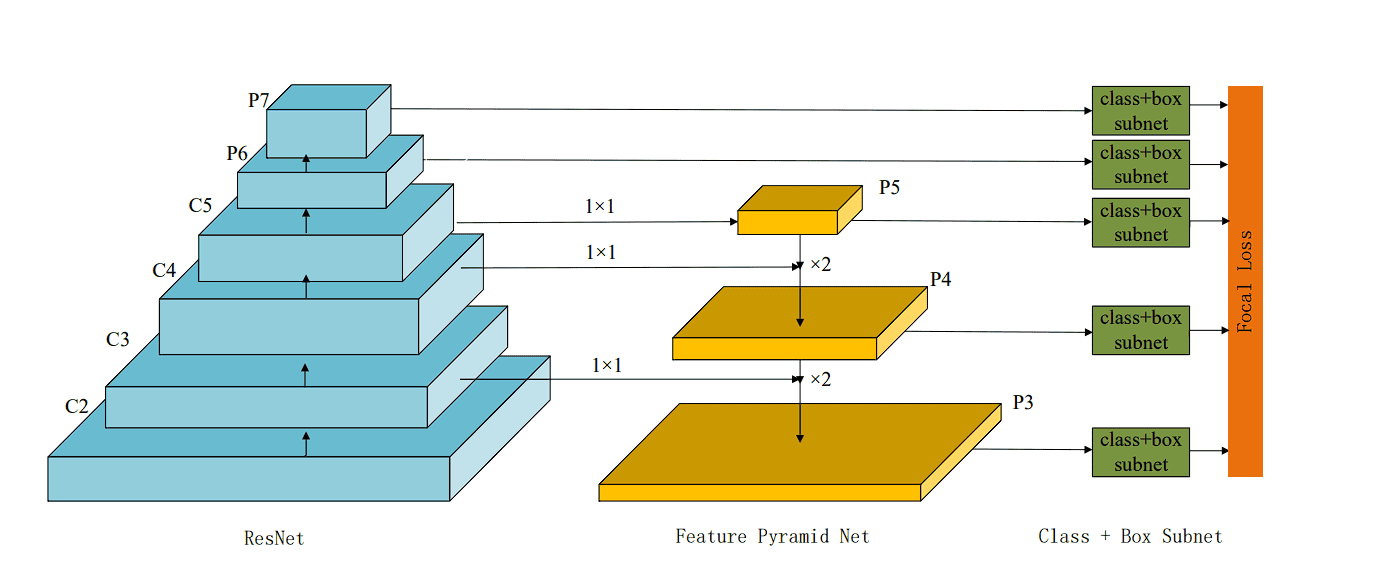
\includegraphics[width=0.9\linewidth]{Figures/Chapter 1/Chapter_3.png}
    \caption{Kiến trúc phương pháp RetinaNet.}
    \label{fig:RetinaNet_architecture}
\end{figure}

Về mặt ưu điểm, RetinaNet đạt được sự cân bằng lý tưởng khi sở hữu độ chính xác cao tiệm cận với các mô hình hai giai đoạn phức tạp như Faster R-CNN, nhưng vẫn duy trì được tốc độ xử lý nhanh chóng của một bộ dò một giai đoạn nhờ cấu trúc không cần vùng đề xuất. Điều này giúp mô hình nhận diện tốt các chướng ngại vật đa dạng trên đường phố ngay cả trong điều kiện mật độ giao thông đông đúc. Tuy nhiên, nhược điểm của RetinaNet là cấu trúc mạng kim tự tháp đặc trưng đi kèm với cơ chế Focal Loss vẫn đòi hỏi một lượng tài nguyên tính toán nhất định ở giai đoạn huấn luyện và có thể gặp hiện tượng giảm tốc độ nhẹ trên các vi điều khiển công suất thấp nếu không được tối ưu hóa hoặc nén mô hình một cách hợp lý.

Tổng kết lại, việc phân tích các đặc điểm kiến trúc của Faster R-CNN, SSD và RetinaNet mang lại cái nhìn toàn diện về sự đánh đổi giữa tốc độ và độ chính xác trong bài toán thị giác máy tính. Đây chính là nền tảng lý thuyết vững chắc giúp định hình và xây dựng một phương pháp nhận diện tối ưu, có khả năng xử lý mượt mà trong thời gian thực nhưng vẫn bảo đảm độ chính xác tối đa để bảo vệ an toàn cho người khiếm thị.

\section{Phương pháp đề xuất}

Trong đề tài này, phương pháp đề xuất tập trung vào việc xây dựng phương pháp hỗ trợ
điều hướng thông minh dành cho người khiếm thị thông qua việc kết hợp nhiều mô hình
trí tuệ nhân tạo trong cùng một pipeline. Hệ thống sử dụng camera
để thu nhận dữ liệu hình ảnh từ môi trường xung quanh, sau đó thực hiện nhận diện vật
cản, theo dõi đối tượng, ước lượng khoảng cách và cảnh báo nguy hiểm bằng giọng nói.

Kiến trúc tổng thể của phương pháp được xây dựng theo hướng xử lý song song nhằm
tăng tốc độ xử lý và đảm bảo khả năng hoạt động thời gian thực. Dữ liệu đầu vào có thể
là hình ảnh, video hoặc luồng camera trực tiếp. Sau khi dữ liệu được đưa vào hệ thống,
quá trình xử lý sẽ được chia thành nhiều giai đoạn khác nhau.

Đầu tiên, mô hình YOLO26 được sử dụng để thực hiện bài toán nhận diện vật cản.
Mô hình có nhiệm vụ phát hiện các đối tượng xuất hiện trong khung hình như người đi
bộ, xe máy, ô tô hoặc các chướng ngại vật khác. YOLO26 được lựa chọn do có khả năng
xử lý nhanh và phù hợp với các ứng dụng thời gian thực. Ngoài ra, mô hình được fine-tune
trên tập dữ liệu phù hợp nhằm nâng cao độ chính xác trong môi trường thực tế.

Song song với quá trình nhận diện đối tượng, hệ thống sử dụng mô hình MiDaS để
thực hiện bài toán Monocular Depth Estimation. Mô hình này cho phép ước lượng độ sâu
và khoảng cách của vật thể chỉ từ một camera đơn mà không cần sử dụng camera stereo
hoặc cảm biến chuyên dụng. Kết quả của MiDaS là bản đồ độ sâu (Depth Map), thể hiện
mức độ gần hoặc xa của các vật thể trong không gian.

Sau khi phát hiện đối tượng, hệ thống sử dụng thuật toán ByteTrack để thực hiện
theo dõi đa đối tượng (Multi-Object Tracking). ByteTrack có nhiệm vụ gán ID cho từng
đối tượng và duy trì việc theo dõi xuyên suốt nhiều khung hình liên tiếp. Điều này giúp
hệ thống xác định được hướng di chuyển cũng như trạng thái thay đổi của vật cản theo
thời gian thực.

Kết quả từ YOLO26, MiDaS và ByteTrack được đưa vào Fusion Pipeline để tổng
hợp thông tin. Tại đây, hệ thống kết hợp thông tin về loại đối tượng, vị trí, hướng di
chuyển và khoảng cách nhằm phân tích mức độ nguy hiểm của từng vật cản đối với
người dùng.

Dựa trên kết quả phân tích, hệ thống Danger Analyzer sẽ xác định mức độ cảnh báo
phù hợp. Nếu phát hiện vật cản nguy hiểm hoặc đối tượng đang di chuyển đến gần người
dùng, hệ thống sẽ sinh nội dung cảnh báo tương ứng.

Cuối cùng, hệ thống sử dụng Text-to-Speech (TTS) tiếng Việt thông qua gTTS hoặc
eSpeak để chuyển nội dung cảnh báo thành giọng nói. Cảnh báo âm thanh được phát theo
thời gian thực nhằm hỗ trợ người khiếm thị nhận biết môi trường xung quanh và nâng
cao độ an toàn trong quá trình di chuyển.

Ngoài ra, hệ thống còn được triển khai với FastAPI và WebSocket ở phía backend
nhằm hỗ trợ xử lý ảnh/video và truyền dữ liệu thời gian thực. Giao diện frontend được
xây dựng bằng React và Vite, giúp hiển thị trực quan kết quả nhận diện và hỗ trợ quản lý
toàn bộ hệ thống.
